\documentclass[border=1cm]{standalone}

\usepackage{tikz}
\usepackage{xcolor}

\begin{document}
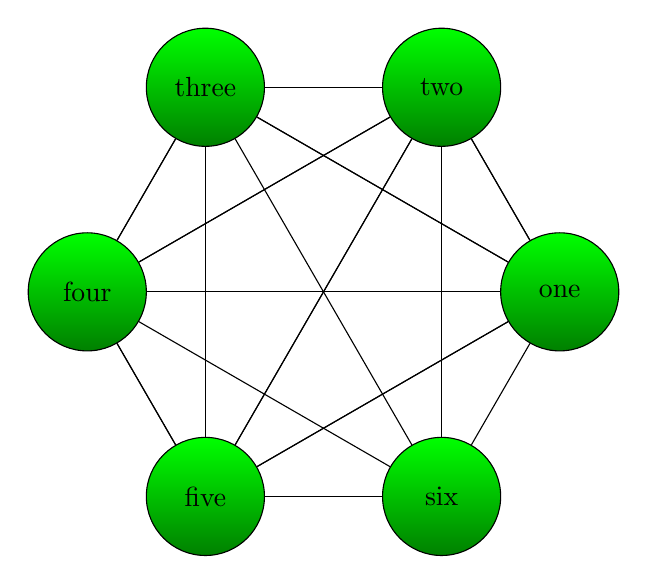
\begin{tikzpicture}
    \foreach \x /\alph/\name in {0/a/one, 60/b/two, 120/c/three, 180/d/four, 240/e/five, 300/f/six}{
    \node[circle, fill=green,minimum width=15mm,draw,shading=axis,top color=green, bottom color=green!50!black] (\alph) at (\x:3cm) {\name}; }

    \foreach \alpha in {a,b,c,d,e,f}%
    {%
    \foreach \alphb in {a,b,c,d,e}%
    {%
    \draw (\alpha) -- (\alphb);%
    }}
 \end{tikzpicture}


\end{document}